\documentclass[]{article}

% Imported Packages
%------------------------------------------------------------------------------
\usepackage{amssymb}
\usepackage{amstext}
\usepackage{amsthm}
\usepackage{amsmath}
\usepackage{enumerate}
\usepackage{fancyhdr}
\usepackage[margin=1in]{geometry}
\usepackage{graphicx}
\usepackage{longtable}
%\usepackage{extarrows}
%\usepackage{setspace}
%\usepackage{xcolor}
\usepackage{color}
%------------------------------------------------------------------------------

% Header and Footer
%------------------------------------------------------------------------------
\pagestyle{plain}  
\renewcommand\headrulewidth{0.4pt}                                      
\renewcommand\footrulewidth{0.4pt}                                    
%------------------------------------------------------------------------------

% Title Details
%------------------------------------------------------------------------------
\title{Deliverable \#1: Software Requirement Specification (SRS)}
\author{SE 3A04: Software Design III -- Large System Design}
\date{}
                            
%------------------------------------------------------------------------------

% Document
%------------------------------------------------------------------------------
\begin{document}

\maketitle	
\noindent{\bf Tutorial Number:} T01\\
{\bf Group Number:} G01 \\
{\bf Group Members:} 
\begin{itemize}
	\item Benjamin Bloomfield
	\item Vikram Chandar
    \item Trisha Panchal
    \item Yug Vashisth
    \item Hamza Nadeem
\end{itemize}

\section*{IMPORTANT NOTES}
\begin{itemize}
	\item Be sure to include all sections of the template in your document regardless whether you have something to write for each or not
	\begin{itemize}
		\item If you do not have anything to write in a section, indicate this by the \emph{N/A}, \emph{void}, \emph{none}, etc.
	\end{itemize}
	\item Uniquely number each of your requirements for easy identification and cross-referencing
	\item Highlight terms that are defined in Section~1.3 (\textbf{Definitions, Acronyms, and Abbreviations}) with \textbf{bold}, \emph{italic} or \underline{underline}
	\item For Deliverable 1, please highlight, in some fashion, all (you may have more than one) creative and innovative features. Your creative and innovative features will generally be described in Section~2.2 (\textbf{Product Functions}), but it will depend on the type of creative or innovative features you are including.
\end{itemize}

\newpage
\section{Introduction}
\label{sec:introduction}
This Software Requirements Specification (SRS) defines the requirements for the Smart City Environmental Monitoring \& Alert System (\textbf{SCEMAS}), a cloud-based platform for smart-city environmental monitoring and alerting. \textbf{SCEMAS} collects real-time environmental telemetry from a distributed sensor network, ingests it through an \textbf{MQTT}-based interface, validates incoming messages, and stores the data for both real-time and historical analysis. The platform aggregates readings, evaluates configurable threshold rules, and generates alerts to support timely city response. \textbf{SCEMAS} provides a secure operator dashboard for visualization and exposes a read-only REST API that returns aggregated, non-sensitive environmental data for public and third-party consumption. This document establishes the system scope, key stakeholders and users, core capabilities, and the constraints and quality attributes that guide implementation and verification.


\subsection{Purpose}
\label{sub:purpose}
% Begin SubSection
This document is used to establish the requirements, performance, and intended behaviour/uses of \textbf{SCEMAS}.
The intended audience of the SRS is the stakeholders of \textbf{SCEMAS}, including developers and testers.
% End SubSection

\subsection{Scope}
\label{sub:scope}
% Begin SubSection
\textbf{SCEMAS} is a cloud-based software product designed to collect, process, store, and distribute environmental telemetry data for urban monitoring and decision support. The system takes real-time data from a distributed network of environmental sensors, including air quality, temperature, humidity, and other environmental indicators. \textbf{SCEMAS} validates, aggregates, and persistently stores this telemetry in a secure database that supports both real-time and historical analysis. The software detects threshold violations and adverse environmental conditions and provides automated alerting functionalities for city operators. A secure dashboard allows authorized city personnel to visualize sensor data on maps and charts, monitor system health, and manage active alerts. Access to system functionality is controlled through a role-based access control (\textbf{RBAC}) framework to ensure that administrative and operational privileges are properly restricted. All telemetry and user data transmitted within the system is encrypted using industry-standard protocols, and stored data is protected through appropriate encryption mechanisms to maintain confidentiality and integrity. The scope of this project focuses on the architectural design and core software services of the system, including telemetry ingestion pipelines, secure data storage, alert evaluation logic, and the protected user interface. Physical sensor hardware, large-scale deployment, and advanced predictive analytics are outside the scope of the initial implementation.
% End SubSection

\subsection{Definitions, Acronyms, and Abbreviations}
\label{sub:definitions_acronyms_and_abbreviations}
% Begin SubSection
\begin{itemize}

	\item \textbf{SCEMAS}: Smart City Environmental Monitoring and Alert System
    \item \textbf{MQTT}: Message Queuing Telemetry Transport
    \item \textbf{CESI}: Canadian Environmental Sustainability Indicators
    \item \textbf{RBAC}: Role-based Access Control
    \item \textbf{PIPEDA}: Personal Information Protection and Electronic Documents Act
    \item \textbf{IoT}: Internet of Things
    \item \textbf{PII}: Personally Identifiable Information

\end{itemize}
% End SubSection

\subsection{References}
\label{sub:references}
% Begin SubSection

\renewcommand{\refname}{} % removes the Reference title
\vspace{-2.5em}
\bibliographystyle{IEEEtran}
\bibliography{references}
% End SubSection

\subsection{Overview}
\label{sub:overview}
The remainder of this Software Requirements Specification (SRS) is organized as follows. Section 2 provides an overall description of \textbf{SCEMAS}, including its context, major functions, intended users, constraints, and assumptions. Section 3 presents the system's use case diagram. Section 4 outlines the functional requirements using the main business events and viewpoint-based scenarios, ending with a consolidated global scenario. Section 5 describes the non-functional requirements, including usability, performance, operational/environmental constraints, maintainability/support, security, cultural/political, and legal considerations. Finally, the Appendix includes the division of labour and any supporting material required by the course template.
% End SubSection

% End Section
\newpage
\section{Overall Product Description}
\label{sec:overall_description}
% Begin Section

\subsection{Product Perspective}
\label{sub:product_perspective}
% Begin SubSection

\textbf{SCEMAS} is a cloud-native \textbf{IoT} software platform built for smart-city environmental monitoring and alerting. It is similar in purpose to Government of Canada environmental dashboards such as the Canadian Environmental Sustainability Indicators (\textbf{CESI}) \cite{cesi} interactive indicators and maps, as well as national monitoring dashboards that report trends and exceedances (for example, water monitoring and wastewater surveillance). However, \textbf{SCEMAS} is designed for city operations where near real-time telemetry ingestion, automated threshold-based alerting, and zone-level aggregation are needed to support fast response and day-to-day decision-making. In many cities, environmental data is tracked in a scattered or manual way, which can slow down responses to issues like poor air quality, heatwaves, or noise disturbances. \textbf{SCEMAS} addresses this by bringing everything into one place: it collects telemetry in real time, automatically detects when conditions cross important thresholds, and shares clear, timely information with both city operators and the public.

At a high level, \textbf{SCEMAS} sits between a network of environmental sensing devices and the people or systems that need environmental insights. During development and testing, the sensors act like real devices by publishing telemetry messages into the platform. Incoming telemetry is accepted through an \textbf{MQTT}-based ingestion entry point, then passed through a validation and ingestion component that checks message structure and plausible value ranges before storing the data in persistent time-series storage.

Once data is stored, \textbf{SCEMAS} performs real-time aggregation to produce useful summaries for monitoring and reporting. A configurable, rule-based alerting engine continuously evaluates these readings and aggregates to detect threshold violations and track alert status over time. When an alert is triggered, \textbf{SCEMAS} can notify external subscriber systems, while also presenting the situation to operators through a secure web dashboard that includes maps, charts, current values, active alerts, system health, and historical trends.

\textbf{SCEMAS} also has a read-only REST API which can be provided to approved third-party organizations upon request. The API returns aggregated, non-sensitive environmental data, and can be paired with a simple demonstration client showing how to consume the endpoints. Potential consumers include mapping applications (e.g., Google Maps overlays) and external organizations that want to display \textbf{SCEMAS} data for their own users or services. To ensure secure administration and accountability, the platform includes \textbf{RBAC} and audit logging across operator-facing functions and administrative actions.

\begin{figure}[h] % h means place here
    \centering
    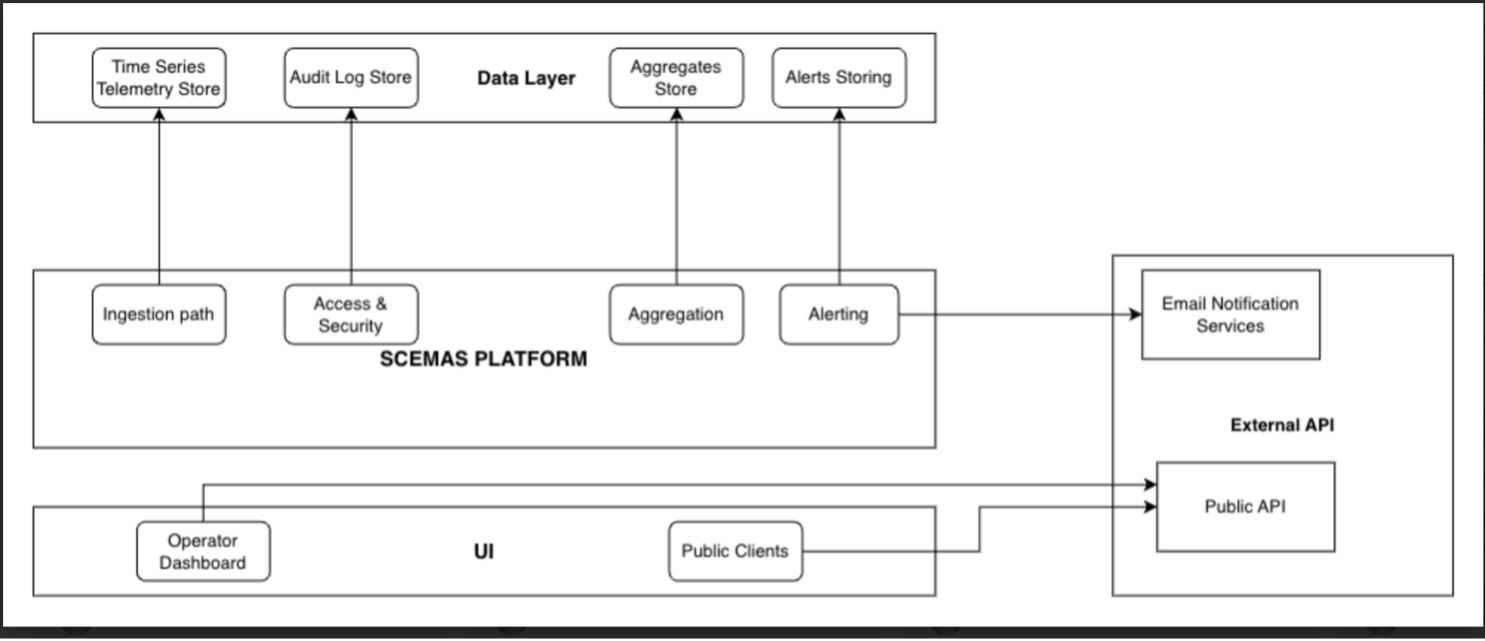
\includegraphics[width=0.95\linewidth]{pictures/F1Block_D.png}
    \caption{\textbf{SCEMAS} high-level block diagram and external interfaces.}
    \label{fig:scemas_block_diagram}
\end{figure}

% End SubSection

\subsection{Product Functions}
\label{sub:product_functions}
% Begin SubSection
\textcolor{red}{The SCEMAS system is divided into 5 working modules, each with its own functionalities. The Alert System module is responsible for handling all alert-related functionality, from defining alert rules to keeping track of the alert log. The User Module handles user account-related events. The Data Handling Module is responsible for handling any data received or transmitted by the system. The Private Dashboard module is responsible for displaying the dashboard for City officials. Lastly, the Public Dashboard Module is responsible for providing a public API for users to access.}
\begin{longtable}{|p{3cm}|p{12cm}|}
\hline
\textbf{Module} & \textbf{Functions} \\
\hline
\endfirsthead

\hline
\textbf{Module} & \textbf{Functions} \\
\hline
\endhead

User Module &
\begin{itemize}
    \item Create an account
        \begin{itemize}
            \item Allow the user to create an account.
        \end{itemize}
    \item Login
        \begin{itemize}
            \item Allow the sign in to their account.
        \end{itemize}
    \item Account Permissions
        \begin{itemize}
            \item Assigns each user with a role controlling their permissions.
        \end{itemize}
    \item Modify Account
        \begin{itemize}
            \item Allow administrators to modify user accounts.
        \end{itemize}
\end{itemize}
\\[5pt]
\hline

Alert System &
\begin{itemize}
    \item Alert Rules
        \begin{itemize}
            \item Allow administrators to define rules based on thresholds.
        \end{itemize}
    \item Evaluate Alert Conditions
        \begin{itemize}
            \item Continuously evaluate incoming data with the defined alert rules.
        \end{itemize}
    \item Alert Triggers
        \begin{itemize}
            \item Trigger an alert upon rule violation.
        \end{itemize}
    \item Alert Status
        \begin{itemize}
            \item Keep a status indicator of each alert between active, acknowledged, or resolved.
        \end{itemize}
    \item Alert Log
        \begin{itemize}
            \item Keep a log of all alerts that occur.
        \end{itemize}
\end{itemize}
\\[5pt]
\hline

Data Handling & 
\begin{itemize}
    \item Receiving data
        \begin{itemize}
            \item Receives \textbf{IoT} data.
        \end{itemize}
    \item Message validation
        \begin{itemize}
            \item Incoming messages are validated for correct format.
        \end{itemize}
    \item Data storage
        \begin{itemize}
            \item All valid data is persistently stored.
        \end{itemize}
    \item Real time aggregation
        \begin{itemize}
            \item Aggregates incoming data into measurements for predefined graphical zones within the city.
        \end{itemize}
\end{itemize}
\\[5pt]
\hline

Private Dashboard & 
\begin{itemize}
    \item Display real-time visualizations
        \begin{itemize}
            \item Display any sensor locations, charts of environmental metrics, etc.
        \end{itemize}
    \item Display real-time visualizations
        \begin{itemize}
            \item Provides overview of system health, active alerts, and access to historical data trends.
        \end{itemize}
    \item Display real-time visualizations
        \begin{itemize}
            \item Ability to manage sensors including adding and deleting them.
        \end{itemize}
    \item Display simulated environmental visualizations
        \begin{itemize}
            \item Ability to observe projected environmental outcomes based on modifications to threshold parameters
        \end{itemize}
\end{itemize}
\\[5pt]
\hline
Public Dashboard & 
\begin{itemize}
    \item Public Rest API
        \begin{itemize}
            \item Exposes aggregated non confidential information for public users.
        \end{itemize}
\end{itemize}
\\[5pt]
\hline
\end{longtable}


% End SubSection

\begin{figure}[h]
    \centering
    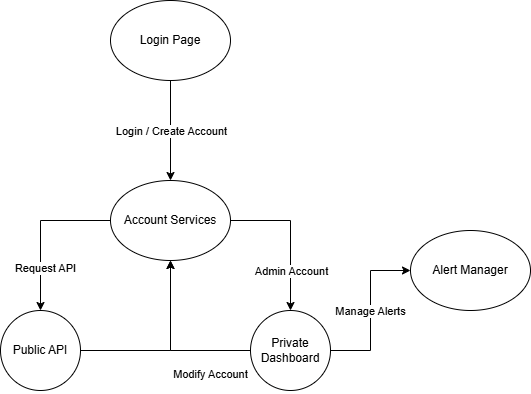
\includegraphics[width=0.7\textwidth]{pictures/2.2state_diagram.png}
    \caption{\textbf{SCEMAS} State Diagram.}
    \label{fig:scemas_state_diagram}
\end{figure}



\subsection{User Characteristics}
\label{sub:user_characteristics}

\subsubsection{User I: City Operators}
City operators analyze the web dashboard to monitor key environmental conditions, and respond accordingly to alerts generated by the system.
\begin{itemize}
    \item \textbf{Education Level}: City operators are expected to have some level of post-secondary education, in environmental science, engineering, urban planning, or another related field of study.
    \item \textbf{Experience}: Prior experience working in a similar role, such as environmental monitoring or public safety operations. Such users should be familiar with interpreting geographical maps, environmental metrics, charts, and trends to identify irregular environmental conditions.
    \item \textbf{Technical Expertise}: City operators are expected to have intermediate computer proficiency, such as the ability to navigate web-based applications, interact with dashboards, and operate data visualization tools.
\end{itemize}

\subsubsection{User II: Public Users}
The general public and citizens can access non-sensitive environmental information through public interfaces that use the read-only REST API, for awareness and safety purposes.
\begin{itemize}
    \item \textbf{Education Level}: Public users are assumed to have basic literacy skills. Basic foundations in listening, reading, writing, and speaking are all the user needs to use the platform without any challenges.
    \item \textbf{Experience}: The user is expected to have little to no prior experience using monitoring systems. The system is designed to be user-friendly to ensure that interactions are straightforward for any user.
    \item \textbf{Technical Expertise}: Basic technical skills, such as understanding how to use a web browser, navigate a webpage, and view digital displays, are all that is necessary.
\end{itemize}

\subsubsection{User III: Administrators}
System administrators are responsible for building and maintaining the system. Their role focuses specifically on ensuring that the system operates securely, behaves correctly, and is maintainable over time.
\begin{itemize}
    \item \textbf{Education Level}: System administrators should have at least a post-secondary education in software engineering, computer science, or another similar technical field.
    \item \textbf{Experience}: They are expected to have prior experience maintaining or managing software systems in a professional or academic setting. This experience includes responsibilities related to access control, system configuration, and operational oversight. Such users should also understand how to define system policies and supervise automated processes such as logging and alert handling. 
    \item \textbf{Technical Expertise}: Advanced technical skills are required for system administrators. They should be familiar with configurable rule-based systems, authentication methods, \textbf{RBAC} models, and audit logging.
\end{itemize}

\subsubsection{User IV: Third-Party Developer}
Third-party developers request and interpret environmental data from the public API to help build external applications. 
\begin{itemize}
    \item \textbf{Education Level}: Developers should have a post-secondary education in software engineering, computer science, or equivalent professional experience.
    \item \textbf{Experience}: The third-party developers are expected to have experience developing software that uses REST APIs and works with JSON data.
    \item \textbf{Technical Expertise}: Proficient technical skills in web application development and API integration, as well as the ability to comprehend API documentation.
\end{itemize}
% End SubSection

\subsection{Constraints}
\label{sub:constraints}
% Begin SubSection

\begin{enumerate}
    \item \textbf{Budget}: The project is constrained by a budget of \$0. This impacts what features the developer can implement, as all technologies, frameworks, cloud services, and other development tools must be free for the team to use.
    \item \textbf{Project Time}: The development of the system is constrained to the Winter 2026 academic calendar. This limits the overall scope of the system, and the amount of features that can be implemented at launch. It shapes the overall development timeline, and the ability to test and optimize. 
    \item \textbf{Communication Protocol}: All sensor telemetry must use the \textbf{MQTT} protocol. This restricts the system's communication model and requires that incoming messages align with the predefined data formats that \textbf{MQTT} messaging supports.
    \item \textbf{Personal Identifiable Information}: The system is constrained to operate under privacy-by-design principles, and must not collect, process, or store any personally identifiable information. Environmental data must be aggregated and associated with general city zones rather than precise locations.
    \item \textbf{Public API Scope}: The public and third-party facing API is constrained to be read-only, meaning that they can not submit data or modify the state. It must only provide access to aggregated, non-sensitive environmental data.
    \item \textbf{Simulated Hardware}: Physical \textbf{IoT} sensor hardware is not available for this project and must be be generated using software simulations. This influences design decisions as the functionality cannot be verified using real-world sensors.
    \item \textbf{Deployment Environment}: The system is constrained to a cloud architecture using available platforms and tools suitable for educational use. Therefore, developers cannot deploy the system on local machines or private servers.
\end{enumerate}
% End SubSection

\subsection{Assumptions and Dependencies}
\label{sub:assumptions_and_dependencies}
% Begin SubSection
\textbf{Assumptions About What the Software Is Aiming to Achieve}
    \begin{itemize}
        \item \textbf{IoT} sensors provide accurate environmental information to the web application.
        \item \textbf{IoT} sensors provide data in real-time.
        \item All telemetry messages follow the predefined \textbf{MQTT} message schema agreed upon by the system.
        \item All \textbf{IoT} sensors have already been installed and require no additional setup.
        \item No \textbf{PII} data will be collected or transmitted by \textbf{IoT} sensors
    \end{itemize}

    \noindent\textbf{Other Assumptions That May Require Requirement Changes if They Fail}
    \begin{itemize}
        \item The selected cloud provider provides sufficient uptime, scalability, and availability for development and deployment.
        \item The System has access to a database capable of efficiently storing and querying time-series data. 
    \end{itemize}


% End SubSection

\subsection{Apportioning of Requirements}
\label{sub:apportioning_of_requirements}
% Begin SubSection
\begin{itemize}
    \item \textbf{Extended language support}: The system will initially be deployed primarily in English. As the platform matures, French language support will be added to align with bilingual expectations for public-sector software in Canada.
    
    \item \textbf{Advanced analytics and forecasting}: The system may incorporate machine learning based prediction of environmental trends in later versions.

    \item \textbf{Integration with emergency response systems}: Integration with municipal emergency services, for automated alerts, will be considered for future releases, once foundational functionality is stable.
\end{itemize}
% End SubSection

% End Section
\newpage
\section{Use Case Diagram}
\label{sec:use_case_diagram}
% Begin Section
\begin{figure}[h]
    \centering
    
\includegraphics[width=0.95\linewidth]{pictures/use_case.png}
    \caption{\textbf{SCEMAS} Use Case Diagram.}
    \label{fig:scemas_use_case_diagram}
\end{figure}
%% End Section

\newpage
\section{Highlights of Functional Requirements}
\label{sec:functional_requirements}
% Begin Section


\noindent {\bf Main Business Events:} The business events that relate to the system include:
\begin{itemize}
    \item BE1. Define a New Alert Rule For Incoming Hurricane.
    \item BE2. Update an Existing Alert Rule Due to New Pollution Limits.
    \item BE3. Remove or Disable an Alert Rule From the Winter Season Ending.
    \item BE4. System Detects Rule Violation From a Wildfire and Triggers Alert 
    \item BE5. Confirm Alert After Detecting a Rule Violation Due to a Heat Wave.
    \item BE6. Mark the alert as resolved
    \item BE7. Request Access to Public API
    \item BE8. Modify Account
    \item BE9. Create Account
    \item BE10. Login
\end{itemize}


\noindent {\bf Viewpoints:} The viewpoints the system considers include:
\begin{itemize}
    \item VP1. City Operators
    \item VP2. Public Users
    \item VP3. Administrators
    \item VP4. Third Party Developers 
    \item VP5. Environmental Monitoring Department
    \item VP6. IT Support
\end{itemize}

\noindent {\bf Business Events:} 

\begin{enumerate}[{\bf BE1.}]
	\item Define a New Alert Rule For Incoming Hurricane. \#1 \\         
    \textbf{Pre-condition}: The administrator is authenticated and logged into the system. There is no alert rule that already exists for the same threshold.
    
		\begin{enumerate}[{\bf VP1.}]
			\item City Operators \#1 
                \begin{quote}
                    N/A
                \end{quote}
                
			\item Public Users \#2 
				\begin{quote}
				    N/A
				\end{quote}
                
			\item Administrators \#3 \\
				\textbf{Main Success Scenario} 
                    \begin{quote}
                    \begin{enumerate}[1.]
                        \item System displays the dashboard.
                        \item Administrator selects \textit{Manage Alerts} tab
                        \item System displays the existing alert rules, and the option to create a new rule.
                        \item Administrator selects \textit{Create New Alert Rule}.
                        \item System displays the alert rule setup form.
                        \item Administrator enters the new alert rule information.
                        \item Administrator submits the alert rule to be added to the system.
                        \item System validates the form.
                        \item System stores the new alert rule.
                        \item System reports to administrator that the alert has been successfully created.
                    \end{enumerate}
                    \end{quote}
                \textbf{Secondary Scenario} 
                \begin{quote}
                    \begin{description}
                        \item[\textmd{8i.}] System detects invalid or incomplete data.
                        \begin{description}
                            \item[\textmd{8i.1}] System prevents the alert rule from being submitted.
                            \item[\textmd{8i.2}] System displays an error message describing the issue.
                            \item[\textmd{8i.3}] System highlights the section(s) that need to be changed.
                            \item[\textmd{8i.4}] Return to BE1-10.
                        \end{description}
                        \item[\textmd{9i.}] System fails to store the added alert rule.
                        \begin{description}
                            \item[\textmd{9i.1}] System displays an error message that the alert rule could not be created.
                            \item[\textmd{9i.2}] System provides instructions for contacting IT Support.
                        \end{description}
                    \end{description}
                \end{quote}
                
			\item Third-Party Developers \#4 
				\begin{quote}
				    N/A
				\end{quote}
                
			\item Environmental Monitoring Department \#5 \\
                \textbf{Main Success Scenario}
                \begin{quote}
                \begin{enumerate}[1.]
                    \item Environmental Monitoring Department identifies a hurricane is forming nearby.
                    \item Environmental Monitoring Department determines that a new threshold is required to monitor wind conditions in new areas.
                    \item Environmental Monitoring Department submits the updated rule requirements to the administrator
                    \item Administrator reviews and approves the requested changes.
                \end{enumerate}
                \end{quote}

			\item IT Support \#6 
                \item[\textmd{4ii}] System should allow IT Support to restore administrator access after verifying their identity.
                \item[\textmd{13i}] System should provide IT Support with error logs to resolve the alert rule storage failures.
		\end{enumerate}
        
        {\bf Global Scenario:}
        	\begin{quote}
        	    \textbf{Pre-condition}: The administrator is authenticated and logged into the system. There is no alert rule that already exists for the same threshold. \\
                \textbf{Main Success Scenario} 
                    \begin{quote}
                    \begin{enumerate}[1.]
                        \item Environmental Monitoring Department identifies a hurricane is forming nearby.
                        \item Environmental Monitoring Department determines that a new threshold is required to monitor wind conditions 
                        \item Environmental Monitoring Department submits the updated rule requirements to the administrator
                        \item Administrator reviews and approves the requested changes.
                        \item System displays the dashboard.
                        \item Administrator selects \textit{Manage Alerts} tab
                        \item System displays the existing alert rules, and the option to create a new rule.
                        \item Administrator selects \textit{Create New Alert Rule}.
                        \item System displays the alert rule setup form.
                        \item Administrator enters the new alert rule information.
                        \item Administrator submits the alert rule to be added to the system.
                        \item System validates the form.
                        \item System stores the new alert rule.
                        \item System reports to administrator that the alert has been successfully created.
                    \end{enumerate}
                    \end{quote}
                \textbf{Secondary Scenario} 
                \begin{quote}
                    \begin{description}
                        \item[\textmd{12i.}] System detects invalid or incomplete data.
                        \begin{description}
                            \item[\textmd{12i.1}] System prevents the alert rule from being submitted.
                            \item[\textmd{12i.2}] System displays an error message describing the issue.
                            \item[\textmd{12i.3}] System highlights the section(s) that need to be changed.
                            \item[\textmd{12i.4}] Return to BE1-10.
                        \end{description}
                        \item[\textmd{13i.}] System fails to store the added alert rule.
                        \begin{description}
                            \item[\textmd{13i.1}] System displays an error message that the alert rule could not be created.
                            \item[\textmd{13i.2}] System provides instructions for contacting IT Support.
                        \end{description}
                    \end{description}
                \end{quote}
        	\end{quote}
\end{enumerate}

\begin{enumerate}[{\bf BE2.}]
	\item Update an Existing Alert Rule Due to New Pollution Limits. \#2 \\ 
    \textbf{Pre-condition}: There must exist at least one alert rule in the system. The administrator is authenticated and logged into the system.
    
		\begin{enumerate}[{\bf VP1.}]
			\item City Operators \#1 
                \begin{quote}
                    N/A
                \end{quote}
                
			\item Public Users \#2 
				\begin{quote}
				    N/A
				\end{quote}
                
			\item Administrators \#3 \\
				\textbf{Main Success Scenario} 
                    \begin{quote}
                    \begin{enumerate}[1.]
                        \item System displays the dashboard.
                        \item Administrator selects \textit{Manage Alerts} tab
                        \item System displays the existing alert rules.
                        \item Administrator selects an alert rule to update.
                        \item Administrator modifies the alert rule parameters.
                        \item Administrator submits the updated alert rule.
                        \item System validates the updated alert rule.
                        \item System updates the alert rule in the systems database.
                        \item System reports to the administrator that the alert rule has been successfully updated.
                    \end{enumerate}
                    \end{quote}
                \textbf{Secondary Scenario} 
                \begin{quote}
                    \begin{description}
                        \item[\textmd{7i.}] Updated alert information is invalid or incomplete.
                        \begin{description}
                            \item[\textmd{7i.1}] System prevents the updated alert rule from being submitted.
                            \item[\textmd{7i.2}] System displays an error message describing the issue.
                            \item[\textmd{7i.3}] System highlights the section(s) that need to be changed.
                            \item[\textmd{7i.4}] Return to BE2-5.
                        \end{description}
                        \item[\textmd{8i.}] System fails to update the alert rule.
                        \begin{description}
                            \item[\textmd{8i.1}] System displays an error message indicating that the alert rule update failed.
                            \item[\textmd{8i.2}] System provides instructions for contacting IT Support.
                        \end{description}
                    \end{description}
                \end{quote}
                
			\item Third-Party Developers \#4
				\begin{quote}
				    N/A
				\end{quote}
                
			\item Environmental Monitoring Department \#5 \\
                \textbf{Main Success Scenario} 
                \begin{quote}
                \begin{enumerate}[1.]
                    \item Environmental Monitoring Department identifies new pollution limits have been established.
                    \item Environmental Monitoring Department makes a particular threshold adjustment based on new data.
                    \item Environmental Monitoring Department submits the updated rule requirements to the administrator
                    \item Administrator reviews and approves the requested changes.
                \end{enumerate}
                \end{quote}

			\item IT Support \#6
            	\begin{quote}
				    8i. System provides IT Support with error logs to resolve the alert rule update failures.
				\end{quote}

		\end{enumerate}
        
        {\bf Global Scenario:}
        	\begin{quote}
        	    \textbf{Pre-condition}: There must exist at least one alert rule in the system. The administrator is authenticated and logged into the system. \\
                \textbf{Main Success Scenario} 
                    \begin{quote}
                    \begin{enumerate}[1.]
                        \item Environmental Monitoring Department identifies an increase in rainfall in the upcoming season.
                        \item Environmental Monitoring Department makes a particular threshold adjustment based on environmental readings.
                        \item Environmental Monitoring Department submits the updated requirements to the administrator
                        \item Administrator reviews and approves the requested changes.
                        \item System displays the dashboard.
                        \item Administrator selects \textit{Manage Alerts} tab
                        \item System displays the existing alert rules.
                        \item Administrator selects an alert rule to update.
                        \item Administrator modifies the alert rule parameters.
                        \item Administrator submits the updated alert rule.
                        \item System validates the updated alert rule.
                        \item System updates the alert rule in the systems database.
                        \item System reports to the administrator that the alert rule has been successfully updated
                    \end{enumerate}
                    \end{quote}
                \textbf{Secondary Scenario} 
                \begin{quote}
                    \begin{description}
                        \item[\textmd{11i.}] Updated alert information is invalid or incomplete.
                        \begin{description}
                            \item[\textmd{11i.1}] System prevents the updated alert rule from being submitted.
                            \item[\textmd{11i.2}] System displays an error message describing the issue.
                            \item[\textmd{11i.3}] System highlights the section(s) that need to be changed.
                            \item[\textmd{11i.4}] Return to BE2-5.
                        \end{description}
                        \item[\textmd{12i.}] System fails to update the alert rule.
                        \begin{description}
                            \item[\textmd{12i.1}] System displays an error message that that the alert rule update failed.
                            \item[\textmd{12i.2}] System provides instructions for contacting IT Support.
                        \end{description}
                    \end{description}
                \end{quote}
        	\end{quote}
\end{enumerate}

\begin{enumerate}[{\bf BE3.}]
	\item Remove or Disable an Alert Rule From the Winter Season Ending. \#3 \\         
    \textbf{Pre-condition}: There must exist at least one alert rule in the system. The administrator is authenticated and logged into the system.
    
		\begin{enumerate}[{\bf VP1.}]
			\item City Operators \#1 
                \begin{quote}
                    N/A
                \end{quote}
                
			\item Public Users \#2 
				\begin{quote}
				    N/A
				\end{quote}
                
			\item Administrators \#3 \\
				\textbf{Main Success Scenario} 
                    \begin{quote}
                    \begin{enumerate}[1.]
                        \item System displays the dashboard.
                        \item Administrator selects \textit{Manage Alerts} tab
                        \item System displays the existing alert rules.
                        \item Administrator selects an alert rule to remove or disable.
                        \item System prompts the administrator for confirmation.
                        \item Administrator confirms the action.
                        \item System removes or disables the alert rule.
                        \item System reports that the alert has been successfully removed or disabled.
                    \end{enumerate}
                    \end{quote}
                \textbf{Secondary Scenario} 
                \begin{quote}
                    \begin{description}
                        \item[\textmd{6i.}] Administrator cancels the confirmation.
                        \begin{description}
                            \item[\textmd{6i.1}] System does not remove or disable the alert rule.
                            \item[\textmd{6i.2}] System returns to the list of existing alert rules.
                        \end{description}
                        \item[\textmd{7i.}] System fails to remove or disable the alert rule.
                        \begin{description}
                            \item[\textmd{7i.1}] System displays an error message that the action failed.
                            \item[\textmd{7i.2}] System provides instructions for contacting IT Support.
                        \end{description}
                    \end{description}
                \end{quote}
                
			\item Third-Party Developers \#4
				\begin{quote}
				    N/A
				\end{quote}
                
			\item Environmental Monitoring Department \#5 \\
                \textbf{Main Success Scenario} 
                \begin{quote}
                \begin{enumerate}[1.]
                    \item Environmental Monitoring Department determines that seasonal environmental conditions (e.g., snow) have ended.
                    \item Environmental Monitoring Department reviews identifies a threshold that is no longer required.
                    \item Environmental Monitoring Department submits the no longer needed requirements to the administrator
                    \item Administrator reviews and approves the requested changes.
                \end{enumerate}
                \end{quote}

			\item IT Support \#6
                \item[\textmd{7i}] System provides IT Support with system logs to investigate and resolve alert rule removal or disable failures.
		\end{enumerate}
        
        {\bf Global Scenario:}
        	\begin{quote}
        	    \textbf{Pre-condition}: There must exist at least one alert rule in the system. The administrator is authenticated and logged into the system. \\
                \textbf{Main Success Scenario} 
                    \begin{quote}
                    \begin{enumerate}[1.]
                        \item Environmental Monitoring Department determines that seasonal environmental conditions (e.g., snow) have ended.
                        \item Environmental Monitoring Department reviews identifies a threshold that is no longer required.
                        \item Environmental Monitoring Department submits the no longer needed requirements to the administrator
                        \item Administrator reviews and approves the requested changes.
                        \item System displays the dashboard.
                        \item Administrator selects \textit{Manage Alerts} tab
                        \item System displays the existing alert rules.
                        \item Administrator selects an alert rule to remove or disable.
                        \item System prompts user for confirmation.
                        \item Administrator confirms the action.
                        \item System removes or disables the alert rule.
                        \item System reports that the alert has been successfully removed or disabled.
                    \end{enumerate}
                    \end{quote}
                \textbf{Secondary Scenario} 
                \begin{quote}
                    \begin{description}
                        \item[\textmd{11i.}] Administrator cancels the confirmation.
                        \begin{description}
                            \item[\textmd{11i.1}] System does not remove or disable the alert rule.
                            \item[\textmd{11i.2}] System returns to the list of existing alert rules.
                        \end{description}
                        \item[\textmd{12i.}] System fails to remove or disable the alert rule.
                        \begin{description}
                            \item[\textmd{12i.1}] System displays an error message that the action failed.
                            \item[\textmd{12i.2}] System provides instructions for contacting IT Support.
                        \end{description}
                    \end{description}
                \end{quote}
        	\end{quote}
\end{enumerate}

\begin{enumerate}[{\bf BE4.}]
	\item System Detects Rule Violation From a Wildfire and Triggers Alert. \#4 \\         
    \textbf{Pre-condition}: The wildfire violates thresholds. The City Operator is authenticated and logged into the system.
    
		\begin{enumerate}[{\bf VP1.}]
			\item City Operators \#1 \\
                \textbf{Main Success Scenario} 
                    \begin{quote}
                    \begin{enumerate}[1.]
                        \item System detects wildfire proximity within 15 km of city limits.
                        \item System triggers the related alert.
                        \item System sends a high-priority notification to the city operator.
                        \item City operator views the active (triggered) alerts.
                        \item City operator selects the alert from the dashboard.
                        \item System displays the alert details.
                        \item City operator reviews the alert information.
                        \item System logs the acknowledgment with the timestamp and operator ID.
                        \item System notifies subscribed external systems through the dedicated API endpoint..
                    \end{enumerate}
                    \end{quote}
                
			\item Public Users \#2 \\
                \textbf{Main Success Scenario} 
                    \begin{quote}
                    \begin{enumerate}[1.]
                        \item Public users view the wildfire details and recommended safety instructions.
                    \end{enumerate}
                    \end{quote}
                
			\item Administrators \#3 
				\begin{quote}
				    N/A
				\end{quote}
                
			\item Third-Party Developers \#4 \\
                \textbf{Main Success Scenario}
                    \begin{quote}
                    \begin{enumerate}[1.]
                        \item Third-party developers confirm delivery of the alert.
                    \end{enumerate}
                    \end{quote}
                
			\item Environmental Monitoring Department \#5 
				\begin{quote}
				    N/A
				\end{quote}

			\item IT Support \#6 
				\begin{quote}
				    N/A
				\end{quote}
		\end{enumerate}
        
        {\bf Global Scenario:}
        	\begin{quote}
        	    \textbf{Pre-condition}: The wildfire violates thresholds. The City Operator is authenticated and logged into the system. \\
                \textbf{Main Success Scenario} 
                    \begin{quote}
                    \begin{enumerate}[1.]
                        \item System detects wildfire proximity within 15 km of city limits.
                        \item System triggers the related alert.
                        \item System sends a high-priority notification to the city operator.
                        \item City operator views the active (triggered) alerts.
                        \item City operator selects the alert from the dashboard.
                        \item System displays the alert details.
                        \item City operator reviews the alert information.
                        \item System logs the acknowledgment with the timestamp and operator ID.
                        \item System sends a notification through the dedicated API endpoint.
                        \item Third-party developers confirm delivery of the alert.
                        \item Public users view the wildfire details and recommended safety instructions.
                    \end{enumerate}
                    \end{quote}
        	\end{quote}
\end{enumerate}

\begin{enumerate}[{\bf BE5.}]
	\item Confirm Alert After Detecting a Rule Violation Due to a Heat Wave. \#5 \\      
    \textbf{Pre-condition}: An alert has been triggered by a threshold violation and is marked as \textit{Active}. The city operator is authenticated and logged into the system.
    
		\begin{enumerate}[{\bf VP1.}]
			\item City Operators \#1 
                \begin{quote}
                    N/A
                \end{quote}
                
			\item Public Users \#2 
				\begin{quote}
				    N/A
				\end{quote}
                
			\item Administrators \#3 \\
				\textbf{Main Success Scenario} 
                    \begin{quote}
                    \begin{enumerate}[1.]
                        \item System displays the dashboard showing the triggered alerts.
                        \item City operator selects an alert from the dashboard.
                        \item System displays the alert details.
                        \item City operator reviews alert information.
                        \item City operator selects the option to acknowledge the alert.
                        \item System updates the alert status to \textit{Acknowledged}.
                        \item System confirms that the alert has been acknowledged.
                    \end{enumerate}
                    \end{quote}
                \textbf{Secondary Scenario} 
                \begin{quote}
                    \begin{description}
                        \item[\textmd{4i.}] Alert has already been acknowledged by another operator.
                        \begin{description}
                            \item[\textmd{4i.1}] System refreshes the alert status.
                            \item[\textmd{4i.2}] System informs the city operator that the alert is already acknowledged.
                        \end{description}
                        \item[\textmd{5i.}] System fails to update the alert status.
                        \begin{description}
                            \item[\textmd{5i.1}] System displays an error message to city operator.
                            \item[\textmd{5i.2}] Alert remains in \textit{Active} status.
                            \item[\textmd{5i.3}] System provides instructions for contacting IT Support.
                        \end{description}
                    \end{description}
                \end{quote}
                
			\item Third-Party Developers \#4
				\begin{quote}
				    N/A
				\end{quote}
                
			\item Environmental Monitoring Department \#5
				\begin{quote}
				    N/A
				\end{quote}

			\item IT Support \#6
                \item[\textmd{5i}] System provides IT Support with system logs to investigate and resolve alert acknowledgment issues.
		\end{enumerate}
        
        {\bf Global Scenario:}
        	\begin{quote}
        	    \textbf{Pre-condition}: An alert has been generated by the system and is marked as \textit{Active}. The city operator is authenticated and logged into the system. \\
                \textbf{Main Success Scenario} 
                    \begin{quote}
                    \begin{enumerate}[1.]
                        \item System displays the dashboard showing the triggered alerts.
                        \item City operator selects an alert from the dashboard.
                        \item System displays the alert details.
                        \item City operator selects the option to acknowledge the alert.
                        \item System updates the alert status to \textit{Acknowledged}.
                        \item System confirms that the alert has been acknowledged. 
                    \end{enumerate}
                    \end{quote}
                \textbf{Secondary Scenario} 
                \begin{quote}
                    \begin{description}
                        \item[\textmd{4i.}] Alert got acknowledged by another operator.
                        \begin{description}
                            \item[\textmd{4i.1}] System refreshes the alert status.
                            \item[\textmd{4i.2}] System informs the city operator that the alert is already acknowledged.
                        \end{description}
                        \item[\textmd{5i.}] System fails to update the alert status.
                        \begin{description}
                            \item[\textmd{5i.1}] System displays an error message to city operator.
                            \item[\textmd{5i.2}] Alert remains in \textit{Active} status.
                            \item[\textmd{5i.3}] System provides instructions for contacting IT Support.
                        \end{description}
                    \end{description}
                \end{quote}
        	\end{quote}
\end{enumerate}

\begin{enumerate}[{\bf BE6.}]
	\item City Operator Resolves an Alert \#6 \\      
    \textbf{Pre-condition}: An alert has been generated by the system and has been acknowledged by a city operator. The city operator is authenticated and logged into the system.
    
		\begin{enumerate}[{\bf VP1.}]
			\item City Operators \#1 
                \begin{quote}
                    N/A
                \end{quote}
                
			\item Public Users \#2 
				\begin{quote}
				    N/A
				\end{quote}
                
			\item Administrators \#3 \\
				\textbf{Main Success Scenario} 
                    \begin{quote}
                    \begin{enumerate}[1.]
                        \item System displays the dashboard showing the active alerts.
                        \item City operator selects an alert.
                        \item System displays the alert details.
                        \item City operator marks the alert as resolved.
                        \item System updates the alert status to \textit{Resolved}.
                        \item System records the time and the operators details.
                        \item System moves the alert to the \textit{Completed} page.
                        \item System confirms that the alert has been resolved.
                    \end{enumerate}
                    \end{quote}
                \textbf{Secondary Scenario} 
                \begin{quote}
                    \begin{description}
                        \item[\textmd{4i.}] Alert got resolved by another operator
                        \begin{description}
                            \item[\textmd{4i.1}] System refreshes the alert status.
                            \item[\textmd{4i.2}] System informs the city operator that the alert is already acknowledged.
                        \end{description}
                        \item[\textmd{5i.}] System fails to update the alert status.
                        \begin{description}
                            \item[\textmd{5i.1}] System displays an error message to city operator.
                            \item[\textmd{5i.2}] Alert remains in \textit{Acknowledged} status.
                            \item[\textmd{5i.2}] System provides instructions for contacting IT Support.
                        \end{description}
                    \end{description}
                \end{quote}
                
			\item Third-Party Developers \#4
				\begin{quote}
				    N/A
				\end{quote}
                
			\item Environmental Monitoring Department \#5
				\begin{quote}
				    N/A
				\end{quote}

			\item IT Support \#6
                \item[\textmd{5i}] System provides IT Support with system logs to investigate and resolve alert resolution failures or audit logging issues.
		\end{enumerate}
        
        {\bf Global Scenario:}
        	\begin{quote}
        	    \textbf{Pre-condition}: An alert has been generated by the system and has been acknowledged by a city operator. The city operator is authenticated and logged into the system. \\
                \textbf{Main Success Scenario} 
                    \begin{quote}
                    \begin{enumerate}[1.]
                        \item System displays the dashboard showing the active alerts.
                        \item City operator selects an alert.
                        \item System displays the alert details.
                        \item City operator marks the alert as resolved.
                        \item System updates the alert status to \textit{Resolved}.
                        \item System records the time and the operators details.
                        \item System moves the alert to the \textit{Completed} page.
                        \item System confirms that the alert has been resolved.
                    \end{enumerate}
                    \end{quote}
                \textbf{Secondary Scenario} 
                \begin{quote}
                    \begin{description}
                        \item[\textmd{4i.}] Alert got resolved by another operator
                        \begin{description}
                            \item[\textmd{4i.1}] System refreshes the alert status.
                            \item[\textmd{4i.2}] System informs the city operator that the alert is already acknowledged.
                        \end{description}
                        \item[\textmd{5i.}] System fails to update the alert status.
                        \begin{description}
                            \item[\textmd{5i.1}] System displays an error message to city operator.
                            \item[\textmd{5i.2}] Alert remains in \textit{Acknowledged} status.
                            \item[\textmd{5i.2}] System provides instructions for contacting IT Support.
                        \end{description}
                    \end{description}
                \end{quote}
        	\end{quote}
\end{enumerate}

\begin{enumerate}[{\bf BE7.}]
    \item Request Access to Public API
        \begin{enumerate}[{\bf VP1.}]
            \item City Operators \\
                N/A. City Operators have access to environmental data internally and do not require public API credentials.

            \item Public Users \\
                \textbf{Pre-condition}: User has a registered Public User \textbf{SCEMAS} account and is logged in.\\
                \textbf{Main Success Scenario}
                \begin{quote}
                    \begin{description}
                        \item[\textmd{5i.}] System informs user that public API access is unavailable and that an account modification to a Third-Party Developer account is required.
                        \begin{description}
                            \item[\textmd{5i.1}] System records the rejected request.
                        \end{description}
                    \end{description}
                \end{quote}

            \item Administrators \\
                \textbf{Pre-condition}: User has a registered Administrator \textbf{SCEMAS} account and is logged in viewing admin dashboard.\\
                \textbf{Main Success Scenario}
                \begin{quote}
                    \begin{description}
                        \item[\textmd{6.}] Administrator Views Request
                        \begin{description}
                            \item[\textmd{6.1}] Administrator adds review comments.
                            \item[\textmd{6.2}] Administrator approves the API access request.
                            \item[\textmd{6.3}] System generates API credentials with appropriate rate limits.
                            \item[\textmd{6.4}] System notifies the user that API access has been granted.
                        \end{description}
                    \end{description}
                \end{quote}

                \textbf{Secondary Scenario}
                \begin{quote}
                    \begin{description}
                        \item[\textmd{6i.}] Administrator rejects API access request.
                        \begin{description}
                            \item[\textmd{6i.1}] System records the rejected request.
                            \item[\textmd{6i.2}] System notifies the user that the request has been rejected.
                        \end{description}
                    \end{description}
                \end{quote}

            \item Third-Party Developers \\
                \textbf{Pre-condition}: User has a registered Third-Party Developer \textbf{SCEMAS} account and is logged in.\\
                \textbf{Main Success Scenario}
                \begin{quote}
                    \begin{enumerate}[1.]
                        \item User selects ``Request Public API''.
                        \item System displays the API access request form.
                        \item User enters required information including project name, purpose, organization affiliation, expected request volume, and required endpoints.
                        \item User submits the API access request form.
                        \item System validates the submitted information.
                        \item System stores the API access request record.
                        \item User receives notification of approved API access.
                        \item User opens the notification.
                        \item System displays API credentials and a link to API documentation.
                    \end{enumerate}
                \end{quote}

                \textbf{Secondary Scenario}
                \begin{quote}
                    \begin{description}
                        \item[\textmd{4i.}] System fails to create API access request.
                        \begin{description}
                            \item[\textmd{4i.1}] System displays a link to contact IT support.
                            \item[\textmd{4i.2}] User navigates to the IT support ticket page.
                            \item[\textmd{4i.3}] User creates a support ticket describing the issue.
                            \item[\textmd{4i.4}] User submits the support ticket.
                            \item[\textmd{4i.5}] IT Support responds with remediation instructions.
                            \item[\textmd{4i.6}] User follows instructions and returns to BE6-3.
                        \end{description}
                        \item[\textmd{6i.}] User receives notification that API access request was rejected.
                        \begin{description}
                            \item[\textmd{6i.1}] User opens the rejection notification.
                            \item[\textmd{6i.2}] System displays rejection reason and administrator comments.
                            \item[\textmd{6i.3}] User reviews comments and returns to BE6-1.
                        \end{description}
                    \end{description}
                \end{quote}

            \item Environmental Monitoring Department \\
                N/A.

            \item IT Support \\
    \textbf{Pre-condition}: User has a registered IT Support \textbf{SCEMAS} account and is logged in.\\
    \textbf{Main Success Scenario}
    \begin{quote}
        \begin{description}
            \item[\textmd{4i.}] System fails to submit API access request form.
            \begin{description}
                \item[\textmd{4i.1}] System displays link to customer support page.
            \end{description}
        \end{description}
    \end{quote}


        \end{enumerate}
        {\bf Global Scenario:} \\
                \textbf{Pre-condition}: User has a registered Third-Party Developer \textbf{SCEMAS} account and is logged in.\\
                \textbf{Main Success Scenario}
                \begin{quote}
                    \begin{enumerate}[1.]
                        \item User selects ``Request Public API''.
                        \item System displays the API access request form.
                        \item User enters required project and usage information.
                        \item User submits the API access request form.
                        \item System validates and stores the request.
                        \item Administrator reviews and approves the request.
                        \item System generates API credentials with appropriate rate limits.
                        \item System notifies the user that API access has been granted.
                    \end{enumerate}
                \end{quote}

                \textbf{Secondary Scenario}
                \begin{quote}
                    \begin{description}
                        \item[\textmd{4i.}] System fails to submit API access request form.
                        \begin{description}
                            \item[\textmd{4i.1}] System prompts user to contact IT support.
                        \end{description}

                        \item[\textmd{5i.}] System detects invalid form fields.
                        \begin{description}
                            \item[\textmd{5i.1}] User is prompted to correct the form.
                            \item[\textmd{5i.2}] User resubmits the request.
                        \end{description}

                        \item[\textmd{6i.}] Administrator rejects the request.
                        \begin{description}
                            \item[\textmd{6i.1}] User receives rejection notification.
                            \item[\textmd{6i.2}] User reviews comments and returns to BE6-1.
                        \end{description}
                    \end{description}
                \end{quote}
\end{enumerate}


\begin{enumerate}[{\bf BE8.}]
	\item Modify Account
		\begin{enumerate}[{\bf VP1.}]
			\item City Operators \\
				    N/A. City Operators do not have permission to modify user accounts.

			\item Public Users \\
                \textbf{Pre-condition}: User has a valid Public User \textbf{SCEMAS} account and is logged in. \\
                \textbf{Main Success Scenario}
                \begin{quote}
                    \begin{enumerate}[1.]
                        \item User selects ``Request Account Modification''.
                        \item System displays an account modification page containing a request form.
                        \item User enters the purpose of the request and organization affiliation.
                        \item User submits the account modification request form.
                        \item System records the account modification request.
                        \item System notifies the user of successful account modification decision.
                        \item User opens the notification.
                        \item System displays confirmation of the change, updated permission details, and administrator comments.
                    \end{enumerate}
                \end{quote}
                \textbf{Secondary Scenario}
                \begin{quote}
                    \begin{description}
                        \item[\textmd{3i.}] User submits invalid or incomplete form details.
                        \begin{description}
                            \item[\textmd{3i.1}] System prompts the user to correct the form and retry submission.
                        \end{description}
                        \item[\textmd{4i.}] System prompts user to contact customer support.
                        \item[\textmd{6i.}] User receives a rejection notification.
                        \begin{description}
                            \item[\textmd{6i.1}] User reviews comments and returns to BE8-1.
                        \end{description}
                    \end{description}
                \end{quote}

			\item Administrators \\
                \textbf{Pre-condition}: User has a valid Administrator \textbf{SCEMAS} account and is logged in. \\
                \textbf{Main Success Scenario}
                \begin{quote}
    \begin{description}
        \item[\textmd{5.}] Administrator navigates to the admin dashboard.
        \item[\textmd{6.}] Administrator selects ``View Account Modification Request Tickets''.
        \item[\textmd{7.}] Administrator selects a ticket to view request details.
        \item[\textmd{8.}] Administrator adds review comments.
        \item[\textmd{9.}] Administrator approves the account modification request.
        \item[\textmd{9i.}] Administrator rejects the request.
    \end{description}
\end{quote}


			\item Third-Party Developers \\
                \textbf{Pre-condition}: User has a valid Third-Party Developer \textbf{SCEMAS} account and is logged in. \\
                \textbf{Main Success Scenario}
                \begin{quote}
                    \begin{enumerate}[1.]
                        \item Developer selects ``Request Account Modification''.
                        \item System displays an account modification page containing a request form.
                        \item Developer enters the purpose of the request, organization affiliation, and developer credentials.
                        \item Developer submits the account modification request form.
                        \item System records the account modification request.
                        \item System notifies the developer of the account modification decision.
                        \item Developer opens the notification.
                        \item System displays confirmation of the change, updated permission details, and administrator comments.
                    \end{enumerate}
                \end{quote}
                \textbf{Secondary Scenario}
                \begin{quote}
                    \begin{description}
                        \item[\textmd{3i.}] Developer submits invalid or incomplete form details.
                        \begin{description}
                            \item[\textmd{3i.1}] System prompts the developer to correct the form and retry submission.
                        \end{description}
                        \item[\textmd{4i.}] System prompts developer to contact customer support.
                        \item[\textmd{6i.}] Developer receives a rejection notification.
                        \begin{description}
                            \item[\textmd{6i.1}] Developer reviews comments and returns to BE8-1.
                        \end{description}
                    \end{description}
                \end{quote}

			\item Environmental Monitoring Department \\
				    N/A.

			\item IT Support \\
                \textbf{Pre-condition}: User has a registered IT Support \textbf{SCEMAS} account and is logged in. \\
                \textbf{Main Success Scenario}
                \begin{quote}
    \begin{description}
        \item[\textmd{4i.}] System displays link to customer support page.
        \begin{description}
            \item[\textmd{4i.1}] IT Support navigates to the IT support ticket dashboard.
            \item[\textmd{4i.2}] IT Support selects a support ticket to view details.
            \item[\textmd{4i.3}] IT Support resolves the issue and documents actions taken.
            \item[\textmd{4i.4}] IT Support closes the support ticket.
        \end{description}
    \end{description}
\end{quote}


        
\end{enumerate}
{\bf Global Scenario:}
        \begin{quote}
            \textbf{Pre-condition}: User has a valid Public User or Third-Party Developer \textbf{SCEMAS} account and is logged in. \\
            \textbf{Main Success Scenario}
            \begin{quote}
                \begin{enumerate}[1.]
                    \item User selects ``Request Account Modification''.
                    \item System displays the account modification request form.
                    \item User submits required modification details.
                    \item Administrator reviews the modification request.
                    \item Administrator approves the request.
                    \item System records the account modification.
                    \item System notifies the user of the modification.
                    \item User reviews confirmation and updated permissions.
                \end{enumerate}
            \end{quote}
            \textbf{Secondary Scenario}
            \begin{quote}
                \begin{description}
                    \item[\textmd{3i.}] User submits invalid or incomplete form details.
                    \begin{description}
                        \item[\textmd{3i.1}] User is prompted to retry submission.
                    \end{description}
                    \item[\textmd{4i.}] System prompts user to contact customer support.
                    \item[\textmd{9i.}] Administrator rejects the request.
                    \begin{description}
                        \item[\textmd{9i.1}] User receives rejection notification.
                        \item[\textmd{9i.2}] User reviews comments and returns to BE8-1.
                    \end{description}
                    \end{description}
            \end{quote}
        \end{quote}
\end{enumerate}


\begin{enumerate}[{\bf BE9.}]
	\item Create Account \#9
		\begin{enumerate}[{\bf VP1.}]
			\item City Operators \#1\\
                \textbf{Pre-condition}: User does not have a \textbf{SCEMAS} account and is not logged in. \\
                \textbf{Main Success Scenario}
                \begin{quote}
                    \begin{enumerate}[1.]
                        \item User navigates to the \textbf{SCEMAS} portal
                        \item User selects ``Request Account''
                        \item User selects ``City Operator'' as requested role
                        \item User enters required personal and work-related information
                        \item User submits the account request
                        \item System validates the submitted information
                        \item System creates an account request record
                        \item System displays confirmation that the request has been submitted
                    \end{enumerate}
                \end{quote}
                \textbf{Secondary Scenario}
                \begin{quote}
                    \begin{description}
                        \item[\textmd{6i.}] System detects invalid or missing information
                        \begin{description}
                            \item[\textmd{6i.1}] System displays validation errors
                            \item[\textmd{6i.2}] User corrects information
                            \item[\textmd{6i.2}] User resubmits the request
                        \end{description}
                    \end{description}
                \end{quote}
                        
            \item Public Users \#2\\
                N/A. City Operators do not have permission to modify user accounts.

			\item Administrators \#3\\
                \textbf{Pre-condition}: User has a registered Administrator \textbf{SCEMAS} account and is logged in. \\
                \textbf{Main Success Scenario}
                \begin{quote}
                    \begin{enumerate}[1.]
                        \item Administrator navigates to the administration dashboard
                        \item Administrator selects ``Create User Account''
                        \item Administrator enters user information
                        \item Administrator assigns an access level
                        \item Administrator submits the request
                        \item System validates the information
                        \item System creates the user account
                        \item System logs the administrative action
                    \end{enumerate}
                \end{quote}
                \textbf{Secondary Scenario}
                \begin{quote}
                    \begin{description}
                        \item[\textmd{6i.}] System detects invalid account information
                        \begin{description}
                            \item[\textmd{6i.1}] System displays error message
                            \item[\textmd{6i.2}] Administrator corrects information and resubmits
                        \end{description}
                    \end{description}
                \end{quote}

			\item Third-Party Developers \#4\\
                N/A. Third party developers do not require accounts within the system.

			\item Environmental Monitoring Department \#5\\
                N/A.

			\item IT Support \#6\\
                \textbf{Pre-condition}: IT Support personnel has access to an Administrator account. \\
                \textbf{Main Success Scenario}
                \begin{quote}
                    \begin{enumerate}[1.]
                        \item IT Support navigates to the administration interface
                        \item IT Support selects ``Create User Account''
                        \item IT Support enters account information
                        \item IT Support assigns administrator-level privileges
                        \item IT Support submits the request
                        \item System creates the account
                        \item System logs the action
                    \end{enumerate}
                \end{quote}
		\end{enumerate}
    {\bf Global Scenario:}
        \begin{quote}
            \textbf{Pre-condition}: The user does not have an existing \textbf{SCEMAS} account. Administrators and IT Support personnel must be logged into an authorized administrative account. \\
            \textbf{Main Success Scenario}
            \begin{quote}
                \begin{enumerate}[1.]
                    \item The requester (City Operator, Administrator, or IT Support) navigates to the \textbf{SCEMAS} portal or administrative dashboard.
					\item The system displays available account-creation options appropriate to the requester's role.
					\item The requester selects ``Create Account'' or ``Request Account''.
					\item The requester enters all required personal and work‑related information.
					\item The system validates all submitted information.
					\item The system performs one of the following based on requester type: creates an account request record (City Operator), OR creates a new active user account (Administrator, IT Support).
					\item If created by an Administrator or IT Support, the system logs the administrative action.
					\item The system displays confirmation that the account request or account creation has been successfully submitted.
                \end{enumerate}
            \end{quote}
            \textbf{Secondary Scenarios}
            \begin{quote}
                \begin{description}
                    \item[\textmd{6i.}] Missing or invalid information
                    \begin{description}
                        \item[\textmd{6i.1}] The system detects invalid or incomplete fields.
                        \item[\textmd{6i.2}] The system displays the specific validation errors.
                        \item[\textmd{6i.3}] The requester corrects the information.
                        \item[\textmd{6i.4}] The requester resubmits the request.
                        \item[\textmd{6i.5}] Returns to BE9-5.
                    \end{description}
                    \item[\textmd{6ii.}] System fails to create an account request (City Operator only)
                    \begin{description}
                        \item[\textmd{6ii.1}] The system cannot create the account request record.
                        \item[\textmd{6ii.2}] The system displays an error message indicating the failure.
                        \item[\textmd{6ii.3}] The system prompts the requester to retry the submission.
                        \item[\textmd{6ii.4}] Returns to BE9-4.
                    \end{description}
                    \item[\textmd{6iii.}] System fails to create the account (Administrator or IT Support)
                    \begin{description}
                        \item[\textmd{6iii.1}] The system is unable to create the new account.
                        \item[\textmd{6iii.2}] The system displays an error message describing the issue.
                        \item[\textmd{6iii.3}] The requester may correct any information or attempt submission again.
                        \item[\textmd{6iii.4}] Returns to BE9-4.
                    \end{description}
                \end{description}
            \end{quote}
        \end{quote}
\end{enumerate}

\begin{enumerate}[{\bf BE10.}]
    \item Login \#10
        \begin{enumerate}[{\bf VP1.}]
            \item City Operators \#1\\
                \textbf{Pre-condition}: User has a valid City Operator \textbf{SCEMAS} account.\\
                \textbf{Main Success Scenario}
                \begin{quote}
                    \begin{enumerate}[1.]
                        \item User navigates to the \textbf{SCEMAS} login page
                        \item User enters login credentials
                        \item User clicks ``Sign In''
                        \item System validates credentials
                        \item System redirects user to operator dashboard
                    \end{enumerate}
                \end{quote}
                \textbf{Secondary Scenario}
                \begin{quote}
                    \begin{description}
                        \item[\textmd{4i.}] Credentials are incorrect
                        \begin{description}
                            \item[\textmd{4i.1}] System displays authentication failure message
                            \item[\textmd{4i.2}] User retries login
                        \end{description}
                        \item[\textmd{4ii.}] User account does not exist
                        \begin{description}
                            \item[\textmd{4ii.1}] System displays account not found message
                        \end{description}
                    \end{description}
                \end{quote}

            \item Public Users \#2\\
                N/A.

            \item Administrators \#3\\
                \textbf{Pre-condition}: User has a valid Administrator \textbf{SCEMAS} account.\\
                \textbf{Main Success Scenario}
                \begin{quote}
                    \begin{enumerate}[1.]
                        \item Administrator navigates to the login page
                        \item Administrator enters credentials
                        \item Administrator submits login request
                        \item System authenticates credentials
                        \item System redirects administrator to admin dashboard
                    \end{enumerate}
                \end{quote}
                \textbf{Secondary Scenario}
                \begin{quote}
                    \begin{description}
                        \item[\textmd{4i.}] Authentication fails
                        \begin{description}
                            \item[\textmd{4i.1}] System denies access
                            \item[\textmd{4i.2}] Administrator retries login
                        \end{description}
                    \end{description}
                \end{quote}

            \item Third-Party Developer \#4\\
                N/A.

            \item Environmental Monitoring Department \#5\\
                N/A.

            \item IT Support \#6\\
                \textbf{Pre-condition}: IT Support has a valid Administrator \textbf{SCEMAS} account.\\
                \textbf{Main Success Scenario}
                \begin{quote}
                    \begin{enumerate}[1.]
                        \item IT Support navigates to the login page
                        \item IT Support enters credentials
                        \item IT Support submits login request
                        \item System authenticates user
                        \item System redirects IT Support to admin dashboard
                    \end{enumerate}
                \end{quote}
                \textbf{Secondary Scenario}
                \begin{quote}
                    \begin{description}
                        \item[\textmd{4i.}] Invalid credentials
                        \begin{description}
                            \item[\textmd{4i.1}] System denies login
                            \item[\textmd{4i.2}] IT Support retries authentication
                        \end{description}
                    \end{description}
                \end{quote}
        \end{enumerate}

    {\bf Global Scenario:}
        \begin{quote}
            \textbf{Pre-condition}: User must have a valid \textbf{SCEMAS} account for their respective role (City Operator, Administrator, or IT Support). User is not currently logged into the system.\\
            \textbf{Main Success Scenario}
            \begin{quote}
                \begin{enumerate}[1.]
                    \item The user (City Operator, Administrator, or IT Support) navigates to the \textbf{SCEMAS} login page.
                    \item The user enters their login credentials.
                    \item The user submits the login request by selecting ``Sign In''.
                    \item The system validates the submitted credentials.
                    \item The system redirects the authenticated user to the appropriate dashboard: Operator Dashboard for City Operators, OR Admin Dashboard for Administrators and IT Support.
                \end{enumerate}
            \end{quote}
            \textbf{Secondary Scenarios}
            \begin{quote}
                \begin{description}
                    \item[\textmd{4i.}] Invalid or incorrect credentials
                    \begin{description}
                        \item[\textmd{4i.1}] The system displays an authentication failure message.
                        \item[\textmd{4i.2}] The user retries login.
                        \item[\textmd{4i.3}] Returns to BE10-2.
                    \end{description}

                    \item[\textmd{4ii.}] Account does not exist (City Operator scenario)
                    \begin{description}
                        \item[\textmd{4ii.1}] The system displays an ``Account not found'' message.
                        \item[\textmd{4ii.2}] Login attempt ends.
                    \end{description}

                    \item[\textmd{4iii.}] Authentication fails (Administrator or IT Support)
                    \begin{description}
                        \item[\textmd{4iii.1}] The system denies access due to authentication failure.
                        \item[\textmd{4iii.2}] The user retries login.
                        \item[\textmd{4iii.3}] Returns to BE10-2.
                    \end{description}
                \end{description}
            \end{quote}
        \end{quote}
\end{enumerate}

% End Section


% Begin Section
\newpage
\section{Non-Functional Requirements}
\label{sec:none-functional_requirements}

% Begin Section
\subsection{Look and Feel Requirements}
\label{sub:look_and_feel_requirements}
% Begin SubSection

\subsubsection{Appearance Requirements}
\label{ssub:appearance_requirements}
% Begin SubSubSection
\begin{enumerate}[{LF-A}1. ]
	\item The system shall use a cool, non-distracting background that does not draw visual focus away from the operational dashboard content.\\
	\textbf{Rationale:} \textbf{SCEMAS} is intended for monitoring environmental conditions. A background with colours that are not warm such as bright red/yellow ensures that users' attention is reserved for critical dashboard elements such as metrics, dashboards, and alerts.
	\item The system should use a consistent font family across all screens.\\
	\textbf{Rationale:} A standardized font enhances the user experience by providing a consistent experience across all screens making it easier to navigate.
	\item Visual alert indicators shall be designed to clearly stand out from non-critical information.\\
	\textbf{Rationale:} Environmental alerts often require immediate action. Distinct visual indicators ensure that critical conditions are quickly recognizable, even when operators are monitoring large volumes of data.
	\item The system shall use a font size that is readable; the font size should also be consistent across all screens relative to the header type.\\
	\textbf{Rationale:} This ensures that information can be categorized into classes such as title, heading, paragraph heading and paragraph body while being readable to users.
\end{enumerate}
% End SubSubSection

\subsubsection{Style Requirements}
\label{ssub:style_requirements}
% Begin SubSubSection
\begin{enumerate}[{LF-S}1. ]
	\item The system shall adapt its layout to different screen resolutions.\\
	\textbf{Rationale:} City operators may access the system from devices with varying screen sizes. Responsive layout behavior ensures a consistent experience across supported devices.
	\item The system shall use a consistent layout that is the same for all dashboard views.\\
	\textbf{Rationale:} A consistent layout structure helps users build familiarity with the interface, preventing unnecessary navigation or relearning on every new screen.
	\item The system shall group related information and controls using spacing, alignment, and section boundaries.\\
	\textbf{Rationale:} Clear visual grouping improves information organization and allows users to quickly identify related data.
	\item The system shall limit the text density on each screen.\\
	\textbf{Rationale:} Screens should be informative and require as little navigation as possible but not overwhelm the user with information cluttering the user experience.
\end{enumerate}
% End SubSubSection

% End SubSection


\subsection{Usability and Humanity Requirements}
\label{sub:usability_and_humanity_requirements}
% Begin SubSection

\subsubsection{Ease of Use Requirements}
\label{ssub:ease_of_use_requirements}
% Begin SubSubSection
\begin{enumerate}[{UH-EOU}1. ]
	\item The system should show brief tooltips for all major controls, indicators and buttons.\\
	\textbf{Rationale:} Giving tooltips enhances user understanding and provides context for each element on the dashboard.
	\item The system should allow users to report bugs to IT support.\\
	\textbf{Rationale:} If users encounter a problem they should be able to receive a response from the \textbf{SCEMAS} team to address their issue and implement fixes.
	\item The system should maintain consistent terminology and terms throughout the interface.\\
	\textbf{Rationale:} Consistent terminology improves learnability and prevents inconsistent descriptions across multiple screens.
	\item The system shall cache user interface preferences, such as selected dashboards or view settings.\\
	\textbf{Rationale:} A cache on the preference allows users to have a consistent configuration in which they view the dashboard which makes the screens tailor made for any particular user.
	\item The system shall contain a Frequently Asked Question section.\\
	\textbf{Rationale:} An FAQ section allows users to get quick and easy answers to commonly asked questions reducing the time required to get acclimated to the system \cite{murphy2025}.
\end{enumerate}
% End SubSubSection

\subsubsection{Personalization and Internationalization Requirements}
\label{ssub:personalization_and_internationalization_requirements}
% Begin SubSubSection
\begin{enumerate}[{UH-PI}1. ]
	\item The system shall allow users to configure personal interface preferences.\\
	\textbf{Rationale:} Allowing users to change their default views, dashboard preference and interface preferences will help increase usability among users.
	\item The system shall allow users to change their language preferences.\\
	\textbf{Rationale:} All users should be able to understand the information on the screen. This is essential for all users to be able to view the system equally and accurately.
	\item The system shall support internationalized measurement units, date formats and time zones.\\
	\textbf{Rationale:} Environmental data must be able to be measured and accessed across all time zones. Supporting international viewing standards ensure data is accessible to people regardless of their location.
\end{enumerate}
% End SubSubSection

\subsubsection{Learning Requirements}
\label{ssub:learning_requirements}
% Begin SubSubSection
\begin{enumerate}[{UH-L}1. ]
	\item Users shall be able to learn how to navigate the main dashboard and interpret key environmental metrics within 20 minutes of first use.\\
	\textbf{Rationale:} Operators must quickly understand the core interface to respond to environmental events effectively. Limiting the learning time ensures the system is intuitive and reduces onboarding effort. \textcolor{red}{\cite{UHL1}}
	\item Users shall be able to configure personal preferences, such as measurement units, default dashboards, and theme settings, within 10 minutes of first use.\\
	\textbf{Rationale:} Users should quickly learn how best to tailor the application to them. If they are able to personalize the system quickly it will make sure that the rest of their time using the system is more enjoyable. \textcolor{red}{\cite{UHL2}}
    \item A trained city operator (someone that has 10+ hours of education on the system) must be able to log into the dashboard and successfully acknowledge a critical environmental alert within 30 seconds of the alert appearing.\\
	\textbf{Rationale:} City operators that are familiar with the system should be able to navigate the dashboard and acknowledge an alert, this shows the system is user-friendly and accessible. \textcolor{red}{\cite{UHL3}}
    \item A trained developer (someone that has 4+ years of experience developing) must be able to understand the API documentation within a 1 hour time frame.\\
	\textbf{Rationale:} Developers that are willing to subscribe to APIs should be able to understand the documentation in the short(1-hour) time frame. If they are able to understand the documentation within this time it means that the documentation is written clearly and helps improve usability of the service. \textcolor{red}{\cite{UHL4}}

\end{enumerate}
% End SubSubSection

\subsubsection{Understandability and Politeness Requirements}
\label{ssub:understandability_and_politeness_requirements}
% Begin SubSubSection
\begin{enumerate}[{UH-UP}1. ]
	\item The system shall use professional and neutral wording in all user-facing communications.\\
	\textbf{Rationale:} Maintaining a professional tone is important to ensure users are not offended by any terminology and allows users to strictly focus on the data.
	\item The system shall avoid technical jargon or abbreviations in messages unless universally understood by target users.\\
	\textbf{Rationale:} Using understandable and general knowledge ensures users of all levels of technicality can understand the information \cite{moran2023}. This prevents confusion and ensures understandability.
\end{enumerate}
% End SubSubSection

\subsubsection{Accessibility Requirements}
\label{ssub:accessibility_requirements}
% Begin SubSubSection
\begin{enumerate}[{UH-A}1. ]
	\item The system shall provide text-to-speech functionality for all essential interface elements.\\
	\textbf{Rationale:} Text to speech allows users that are blind or low-vision to interpret environmental data.
	\item The system shall provide captions or transcripts for all audio content, including notifications and messages.\\
	\textbf{Rationale:} Users who are deaf or hard-of-hearing should be able to  access spoken information like any other able user and a viable way to do this is using text-to-speech \cite{voxpow2020}.
	\item The system shall use a color palette that is accessible to users with common forms of color vision deficiency.\\
	\textbf{Rationale:} City-operated systems must be inclusive and accessible. 1/16 men and 1/240 women have some form of colour deficiency and therefore should be accommodated \cite{davidmath}. Colorblind-friendly design ensures that all operators can correctly interpret system states and alerts without relying solely on colour perception.
\end{enumerate}
% End SubSubSection

% End SubSection


\subsection{Performance Requirements}
\label{sub:performance_requirements}
% Begin SubSection

\subsubsection{Speed and Latency Requirements}
\label{ssub:speed_and_latency_requirements}
% Begin SubSubSection
\begin{enumerate}[{PR-SL}1.]
	\item The web dashboard for city operators should have a load time of less than 1 second. \\
    \textbf{Rationale}: Having a fast-loading website will ensure users remain engaged. A study shows that 40\% of users will leave a website if it takes longer than 3 seconds to load \cite{browserstack}.
    
    \item The system should provide a REST API for public use with a response time of less than 1 second. \\
    \textbf{Rationale}: APIs with lower response time lead to many benefits, like enhancing user satisfaction and increasing cost effectiveness of the system by allowing fewer resources to be used  \cite{farouk2024}. Longer API response times will likely result in user frustration and abandonment \cite{farouk2024}.
\end{enumerate}
% End SubSubSection

\subsubsection{Safety-Critical Requirements}
\label{ssub:safety_critical_requirements}
% Begin SubSubSection
\begin{enumerate}[{PR-SC}1. ]
	\item The system should ensure that alerts are posted in less than 5 seconds of \textcolor{red}{a threshold violation being detected.}\\
    \textbf{Rationale}: A rapid alert system allows operations to respond to any alerts within a timely manner, staging interventions or putting out city-wide alerts where possible. \textcolor{red}{\cite{PRSC1}}
\end{enumerate}
% End SubSubSection

\subsubsection{Precision or Accuracy Requirements}
\label{ssub:precision_or_accuracy_requirements}
% Begin SubSubSection
\begin{enumerate}[{PR-PA}1. ]
	\item For each environmental indicator (air quality, noise levels, temperature, humidity) the system shall have a standard deviation of less than 15\%.\\
    \textbf{Rationale}: Inaccurate data could lead to a false sense of security or a false sense of urgency when trying to address the implications of the measurement \cite{envmon}, its important for the measurement to remain accurate to avoid these situations.
\end{enumerate}
% End SubSubSection

\subsubsection{Reliability and Availability Requirements}
\label{ssub:reliability_and_availability_requirements}
% Begin SubSubSection
\begin{enumerate}[{PR-RA}1. ]
	\item \textcolor{red}{The SCEMAS system should have an uptime of at least 99\%}\\
    \textbf{Rationale}: \textcolor{red}{It is necessary to have an uptime of 99\% to ensure that users have a reliable experience. Lower uptime can lead to a damaged reputation, poor user experience, and loss of trust with users. Therefore, it is important to avoid situations where the system is down for an extended period of time. {\cite{PRRA1a}} {\cite{PRRA1b}}}
    \item The system should ensure that alerts have a false positive rating of less than 1\%\\
    \textbf{Rationale}: A high false positive rating can lead to improper use of resources, impaired efficiency and a loss of trust of users \cite{vwo}. Its important to have a low false positive rate to avoid taking unnecessary measures to correct a false issue.
\end{enumerate}
% End SubSubSection

\subsubsection{Robustness or Fault-Tolerance Requirements}
\label{ssub:robustness_or_fault_tolerance_requirements}
% Begin SubSubSection
\begin{enumerate}[{PR-RFT}1. ]
	\item The System should not fail if one component of it fails.\\
    \textbf{Rationale}: This is to ensure that the system stays functional even if a sensor fails, meaning the system will continue to collect data from the other sensors.
    \item The system should detect and log any errors in under 5 seconds\\
    \textbf{Rationale}: This is to ensure that all errors are properly logged as well as properly addressed within a timely manner \textcolor{red}{\cite{PRRFT2}}.
\end{enumerate}
% End SubSubSection

\subsubsection{Capacity Requirements}
\label{ssub:capacity_requirements}
% Begin SubSubSection
\begin{enumerate}[{PR-C}1. ]
	\item The system should be able handle and store information from at least 150 sensors across the city.\\
    \textbf{Rationale}: A mid sized city requires 150 sensors \cite{english2020} to allow the system to collect accurate data for accurate measurements. Ensuring the whole city is covered allows us to take action where its needed.
\end{enumerate}
% End SubSubSection

\subsubsection{Scalability or Extensibility Requirements}
\label{ssub:scalability_or_extensibility_requirements}
% Begin SubSubSection
\begin{enumerate}[{PR-SE}1. ]
	\item The internal code of our system should follow SOLID design principles to ensure scalability.\\ 
    \textbf{Rationale}: The Solid design principles are a set of principles that help developers write clean, maintainable, and scalable code \cite{gorai2024}. Adopting these principles in the system's design allows our system to be scalable and extensible. 
\end{enumerate}
% End SubSubSection

\subsubsection{Longevity Requirements}
\label{ssub:longevity_requirements}
% Begin SubSubSection
\begin{enumerate}[{PR-L}1. ]
	\item The sensors should use sustainable materials that guarantee a lifespan of at least 2 years\\
    \textbf{Rationale}: \textcolor{red}{Replacing a sensor can be costly and disruptive. It is important that each sensor preforms optimally for an extended period of time to avoid frequent replacements. Replacing a sensor can be costly and disruptive. {\cite{PRL1}}}
\end{enumerate}
% End SubSubSection

% End SubSection

\subsection{Operational and Environmental Requirements}
\label{sub:operational_and_environmental_requirements}
% Begin SubSection

\subsubsection{Expected Physical Environment}
\label{ssub:expected_physical_environment}
% Begin SubSubSection
\begin{enumerate}[{OE-EPE}1. ]
	\item \textbf{SCEMAS} shall operate in a cloud-hosted environment using commodity server infrastructure (virtual machines/containers) and shall not require any specialized physical hardware.\\
    \textbf{Rationale:} The system should be deployable using free-tier or educational cloud resources, and sensor hardware is simulated rather than physically deployed.
    
	\item \textbf{SCEMAS} shall support operation over standard internet connections and tolerate intermittent connectivity from simulated sensor publishers by continuing to run and ingest telemetry once connectivity resumes.\\
    \textbf{Rationale:} \textbf{IoT}-style telemetry publishers may disconnect; the system should remain stable and continue ingesting when publishers reconnect.
\end{enumerate}
% End SubSubSection

\subsubsection{Requirements for Interfacing with Adjacent Systems}
\label{ssub:requirements_for_interfacing_with_adjacent_systems}
% Begin SubSubSection
\begin{enumerate}[{OE-IA}1. ]
	\item \textbf{SCEMAS} shall ingest sensor telemetry through the \textbf{MQTT} protocol and validate each incoming message against a defined schema and plausible value ranges before storage.\\
    \textbf{Rationale:} \textbf{MQTT} ingestion and validation are core requirements for reliable telemetry processing.
    
	\item \textbf{SCEMAS} shall expose a read-only REST API for public/third-party consumption that returns aggregated, non-sensitive environmental data.\\
    \textbf{Rationale:} The public-facing API must be read-only and provide aggregated data rather than sensitive/raw details.
    
	\item When an alert is triggered, \textbf{SCEMAS} shall notify subscribed external systems through a dedicated notification API endpoint.\\
    \textbf{Rationale:} External notifications on alert triggers are a required system capability.
\end{enumerate}
% End SubSubSection

\subsubsection{Productization Requirements}
\label{ssub:productization_requirements}
% Begin SubSubSection
\begin{enumerate}[{OE-P}1. ]
	\item \textbf{SCEMAS} shall provide configuration-driven deployment for thresholds, zone definitions, and alert rules so the same build can be used across environments (dev/test/demo).\\
    \textbf{Rationale:} Configuration-based behavior supports different setups without rebuilding code and better fits a reusable platform.
    
	\item \textbf{SCEMAS} shall include clear operator and developer documentation, including public API documentation sufficient for a competent third-party developer to request and interpret data within two hours.\\
    \textbf{Rationale:} Good documentation is required so external developers can successfully use the API quickly.
\end{enumerate}
% End SubSubSection

\subsubsection{Release Requirements}
\label{ssub:release_requirements}
% Begin SubSubSection
\begin{enumerate}[{OE-R}1. ]
	\item \textbf{SCEMAS} shall support separate deployment profiles for (at minimum) development and demonstration/staging, with distinct configuration for database endpoints, authentication secrets, and rate limits.\\
    \textbf{Rationale:} Separating environments reduces demo risk and avoids mixing secrets/data across deployments.
    
	\item Each \textbf{SCEMAS} release shall be versioned and include a rollback strategy for the dashboard and API services.\\
    \textbf{Rationale:} Cloud deployments can fail; rollback supports service continuity.
\end{enumerate}
% End SubSubSection

% End SubSection


\subsection{Maintainability and Support Requirements}
\label{sub:maintainability_and_support_requirements}
% Begin SubSection

\subsubsection{Maintenance Requirements}
\label{ssub:maintenance_requirements}
% Begin SubSubSection
\begin{enumerate}[{MS-M}1. ]
	\item \textbf{SCEMAS} shall be designed as modular services/components (e.g., ingestion, alerting, storage, dashboard/API) so that changes to one component do not require rewriting unrelated components.\\
    \textbf{Rationale:} Modularity reduces regression risk and makes future extensions (new metrics, new rules) easier.
    
	\item \textbf{SCEMAS} shall maintain automated logs for major runtime events (telemetry ingestion failures, validation rejections, alert triggers, and admin actions) to support debugging and ongoing maintenance.\\
    \textbf{Rationale:} Logs are essential for diagnosing issues in distributed systems and supporting ongoing maintenance.
\end{enumerate}
% End SubSubSection

\subsubsection{Supportability Requirements}
\label{ssub:supportability_requirements}
% Begin SubSubSection
\begin{enumerate}[{MS-S}1. ]
	\item \textbf{SCEMAS} shall provide a support-facing troubleshooting view or documented runbook steps that allow IT Support/Administrators to identify common failures (database unreachable, API rate-limit triggered) and the recommended recovery action.\\
    \textbf{Rationale:} Support needs a fast way to narrow down what broke in a multi-component system (ingestion + storage + dashboards + API).
    
	\item \textbf{SCEMAS} shall provide user-facing error messages on the dashboard/API that are actionable (what happened + what to try next) without exposing sensitive internal details.\\
    \textbf{Rationale:} Clear errors reduce support load, and avoiding internal details supports secure operations.
\end{enumerate}
% End SubSubSection

\subsubsection{Adaptability Requirements}
\label{ssub:adaptability_requirements}
% Begin SubSubSection
\begin{enumerate}[{MS-A}1. ]
	\item \textbf{SCEMAS} shall allow new sensor types/metrics to be introduced by extending the telemetry schema and validation rules, without changing the operator dashboard's core navigation or authentication flow.\\
    \textbf{Rationale:} Monitoring evolves; the system should adapt to new indicators while keeping the operator experience stable.
    
	\item \textbf{SCEMAS} shall be adaptable to multiple deployment providers (or local containers for demos) by avoiding provider-specific hard dependencies in core logic.\\
    \textbf{Rationale:} Teams may switch hosting/deployment options; portability reduces rework.
\end{enumerate}
% End SubSubSection

% End SubSection

\subsection{Security Requirements}
\label{sub:security_requirements}
% Begin SubSection

\subsubsection{Access Requirements}
\label{ssub:access_requirements}
% Begin SubSubSection
\begin{enumerate}[{SR-AC}1. ]
	\item The system must require all users of the dashboard to authenticate using an email/username and password, being granted access to the system. \\
    \textbf{Rationale}: This ensures that only people who are authorized can access the system, which prevents the risk of authorized individuals to alter environmental data \cite{canUserAuth}.

    \item The system must support multi-factor authentication (MFA) for administrative accounts. \\
    \textbf{Rationale}: MFA helps by eliminating the possibility of compromising the credentials of an administrators account. This is crucial, since the administrator is a high-privilege user who can define alert rules, and view sensitive system information \cite{canSecure}.

    \item The system must enforce \textbf{RBAC} to distinguish between the different user groups, such as administrator, city operator, and read-only public users. \\
    \textbf{Rationale}: Enforcing an \textbf{RBAC} policy ensures that each user group can only perform actions that are appropriate to their respective role. This helps to reduce accidental misuse of the systems functions. 

    \item The system must lock out a user account after five consecutive failed login attempts. \\
    \textbf{Rationale}: Protects against repeated attempts of trying to login to an account that does not belong to the respective individual \cite{canUserAuth}.

    \item All \textbf{IoT} devices must be authenticated with a unique key before sending telemetry data to the system. \\
    \textbf{Rationale}: Prevents harmful telemetry to be injection into the system, by limiting entering data to registered and authorized sensors \cite{canIoT}.
\end{enumerate}
% End SubSubSection

\subsubsection{Integrity Requirements}
\label{ssub:integrity_requirements}
% Begin SubSubSection
\begin{enumerate}[{SR-INT}1. ]
    \item Any data transmitted between \textbf{IoT} devices, and the system must be encrypted, and include integrity protection. \\
    \textbf{Rationale}: Ensures that telemetry is protected, and cannot be changed during transmission. As a result, this helps maintain confidentiality and integrity \cite{canEncrypt}.
    
	\item All incoming sensor telemetry must be validated against a defined schema and acceptable value ranges before being stored. \\
    \textbf{Rationale}: Ensures that only correct and meaningful data is allowed to enter the system. This restricts any corrupted/malicious data from affecting any environmental analytics and alerts. 

    \item The system must maintain an audit log to keep track of any data modification, such as alert rule updates, or alert status changes. \\
    \textbf{Rationale}: An audit log is essential to provide traceability to identify any potential modifications made accidentally, or by unauthorized personnel \cite{ali2021}.

    \item The system should use cryptographic hashing for any alert generated, to ensure that the alert data remains secure, and unaltered after generation. \\
    \textbf{Rationale}: Enforces data integrity, and prevents city operators from receiving false notifications \cite{canGuid}.
\end{enumerate}
% End SubSubSection

\subsubsection{Privacy Requirements}
\label{ssub:privacy_requirements}
% Begin SubSubSection
\begin{enumerate}[{SR-P}1. ]
	\item The system will not collect or store any personally identifiable information from public users. \\
    \textbf{Rationale}: Protects individual privacy, and ensures compliance with \textbf{PIPEDA} (Personal Information Protection and Electronic Documents Act) regulations \cite{pipeda}.

    \item The system shall only collect environmental data at the level of general city zones. \\
    \textbf{Rationale}: Ensures citizen privacy by preventing sensor data from tracking individual residents

    \item Public APIs should only provide non-sensitive data to public citizens and third-party developers. \\
    \textbf{Rationale}: Prevents misuse of the API, and protects privacy.
    
\end{enumerate}
% End SubSubSection

\subsubsection{Audit Requirements}
\label{ssub:audit_requirements}
% Begin SubSubSection
\begin{enumerate}[{SR-AU}1. ]
	\item The system shall log all user login attempts, including the timestamp, their distinct identification number, and the location of the request. \\
    \textbf{Rationale}: Ensures accountability for access attempts \cite{english2020}.

    \item The system shall log all access to sensitive data, and data modification such as updating, adding or deleting rule alerts, or registering new sensors or accounts. \\
    \textbf{Rationale}: Ensures sensitive data is properly handled, and traceability of critical changes \cite{secoda2025}.

    \item All audit logs should be retained for at least 1 years. \\
    \textbf{Rationale}: Ensures there is enough time look at incidents, or check compliance \cite{Dreshner2025}.

    \item All audit logs should be protected with access controls to ensure that only authorized security can view or extract information from them. \\
    \textbf{Rationale}: Prevents critical information from being shared without authorization \cite{Dreshner2025}.
    
\end{enumerate}
% End SubSubSection

\subsubsection{Immunity Requirements}
\label{ssub:immunity_requirements}
% Begin SubSubSection
\begin{enumerate}[{SR-IM}1. ]
	\item The system shall keep receiving and storing sensor data even when the real-time processing system is down. \\
    \textbf{Rationale}: Makes sure no sensor data is lost if part of the system stops \cite{canRead}.

    \item The system shall immediately try again when sending sensor data fails.\\
    \textbf{Rationale}: Ensures that sensor data eventually reaches the system, even in the case of network problems \cite{canRead}.
\end{enumerate}
% End SubSubSection

% End SubSection

\subsection{Cultural and Political Requirements}
\label{sub:cultural_and_political_requirements}
% Begin SubSection

\subsubsection{Cultural Requirements}
\label{ssub:cultural_requirements}
% Begin SubSubSection
\begin{enumerate}[{CP-C}1. ]
	\item The system shall not allow users to create an account with an inappropriate or discriminatory name. \\
    \textbf{Rationale}: Prevents harassment, and hate speech, while ensuring that the system remains professional, inclusive and aligned with standards

    \item The system shall not use any symbols, colours, and icons in the dashboards that can be considered offensive based one ones religion, ethnicity, disability or sexual orientation.  \\
    \textbf{Rationale}: Ensures the user interface stays inclusive for a diverse population. Helps reduces the risk of discrimination and reputational damage.
\end{enumerate}
% End SubSubSection

\subsubsection{Political Requirements}
\label{ssub:political_requirements}
% Begin SubSubSection
\begin{enumerate}[{CP-P}1. ]
	\item The system shall comply with all federal, provincial, and municipal regulations regarding environmental monitoring and data sharing \cite{canEnv}. \\
    \textbf{Rationale}: Ensures legal compliance and helps to avoid political conflicts.
    	
    \item The system shall be transparent in how it collects and stores data by giving government authorities access to such data and system reports \cite{canDirective}. \\
    \textbf{Rationale}: Enables accountability to political authorities. 
        	
    \item The system shall provide ways to share environmental data to other authorized groups. \\
    \textbf{Rationale}: Supports collaboration between government organizations.
\end{enumerate}
% End SubSubSection

\subsection{Legal Requirements}
\label{sub:legal_requirements}
% Begin SubSection

\subsubsection{Compliance Requirements}
\label{ssub:compliance_requirements}
% Begin SubSubSection
\begin{enumerate}[{LR-COMP}1. ]
    \item The system shall identify and document the purposes for collection or use of its users' personal information before or at the time of collection. \\
    \textbf{Rationale}: This is \textbf{PIPEDA} Fair Information Principle 2 - Identifying Purposes \cite{pipedaAll}.

    \item The system shall obtain the consent of users for the collection, use, or disclosure of their personal information. \\
    \textbf{Rationale}: This is \textbf{PIPEDA} Fair Information Principle 3 - Consent \cite{pipedaAll}.

    \item The system shall limit any collection of personal information to what is necessary for the stated purposes. \\
    \textbf{Rationale}: This is \textbf{PIPEDA} Fair Information Principle 4 - Limiting Collection \cite{pipedaAll}.

    \item The system shall use, disclose, and retain personal information only for the purposes for which it was collected, and will not retain the information longer than necessary. \\
    \textbf{Rationale}: This is \textbf{PIPEDA} Fair Information Principle 5 - Limiting Use, Disclosure, and Retention \cite{pipedaAll}.

    \item The system shall protect personal information with safeguards appropriate to its sensitivity, and will not store credentials or other sensitive data in unsecured locations. \\
    \textbf{Rationale}: This is \textbf{PIPEDA} Fair Information Principle 7 - Safeguards \cite{pipedaAll}.
\end{enumerate}
% End SubSubSection

\subsubsection{Standards Requirements}
\label{ssub:standards_requirements}
% Begin SubSubSection
\begin{enumerate}[{LR-STD}1. ]
    \item The system shall encrypt all data in transit using current secure protocols. \\
    \textbf{Rationale}: Aligns with Canadian federal guidelines on cryptographic protection and secure network protocol configuration \cite{canEncrypt,secureProtocols}.

    \item The system shall enforce API rate limits, quotas, and bounded payload sizes on all externally reachable endpoints, and shall not allow unbounded request rates. \\
    \textbf{Rationale}: Aligning with recommended API protection standards to prevent resource exhaustion \cite{nistAPI}.

    \item The system shall require strong authentication for protected endpoints, and shall not expose administrative functions without authentication. \\
    \textbf{Rationale}: Consistent with API security standards for authorized access \cite{nistAPI}.
\end{enumerate}
% End SubSubSection

% End SubSection

% End Section
\newpage
\section{Innovative Feature}
\label{sec:innovative_feature}
An innovative feature that could be added is an included simulation feature that would allow city operators to adjust environmental parameters and observe the projected outcome in a visual dashboard overlaid on top of the city. This would help city operators plan response strategies, visualize worst case outcomes, and help train employees without impacting live data.

\newpage
\appendix
\section{Division of Labour}
\label{sec:division_of_labour}
% Begin Section

\noindent \textbf{Benjamin Bloomfield} 
\begin{itemize}
    \item 1.4 References
    \begin{itemize}
        \item Managed all in-text citations.
        \item Formatted each website in IEEE format. 
        \item Organized all citations in the references.bib file.
    \end{itemize}
    \item Revised 2.2 Product Functions as a group.
    \item 2.3 User Characteristics.
    \item 2.4 Constraints.
    \item 4 Highlights of Functional Requirements:
    \begin{itemize}
        \item Helped devise the list of viewpoints.
        \item Wrote the LaTeX code structure for business events.
        \item Wrote BE1-BE6.
    \end{itemize}
    \item Non-Functional Requirements: 5.6, 5.7
    \item Organized storage and display of figures. 
    \item Wrote the LaTeX code structure for Division of Labour

    \vspace{0.5cm}
    \centering
    
\includegraphics[width=10cm]{signatures/ben_bloomfield_signature.jpg}
    \\\vspace{0.2cm}
    Date: February 13, 2025 
    \vspace{0.5cm}

\end{itemize}


\noindent \textbf{Vikram Chandar}
\begin{itemize}
    \item Revised 1.2 Scope and 2.1 Product Perspective
    \item 1.3 Definitions, Acronyms, and Abbreviation
    \item Revised 2.2 Product Functions as a Group
    \item 2.5 Assumptions and Dependencie
    \item Functional Requirements
    \begin{itemize}
        \item Helped create the list of viewpoints as a team
        \item Wrote BE6,BE7.
    \end{itemize}
    \item 5.1 Look and Feel Requirement
    \item 5.2 Style Requirements
    \item 6 - Thought of innovative feature and adapted project around this feature.

    \vspace{0.5cm}
    \centering
    
\includegraphics[width=10cm]{signatures/IMG_4568.jpg}
    \\\vspace{0.2cm}
    Date: February 13, 2025 
    \vspace{0.5cm}
\end{itemize}



\noindent \textbf{Trisha Panchal}
\begin{itemize}
    \item Wrote 1.2 Scope. Revised based on Vikram's feedback during tutorial.
    \item Reviewed 2.1 Product Perspective, and gave Yug feedback on the block diagram during tutorial.
    \item Revised 2.2 Product Functions choice of modules and functions as a group.
    \item Wrote 2.6 Apportioning of Requirements.
    \item Designed 3 Use Case Diagram. Revised after rest of the group reviewed it. Revised to incorporate feedback from TA.
    \item 4 Highlights of Functional Requirements:
    \begin{itemize}
        \item Generated list of business events and viewpoints as a group.
        \item Wrote BE9 Create Account, and BE10 Login.
    \end{itemize}
    \item Wrote 5.8 Legal Requirements.
    \item Reviewed 6 Innovative Feature as a group.

    \vspace{0.5cm}
    \centering
    
\includegraphics[width=10cm]{signatures/trisha_d1_sign.jpg}
    \\\vspace{0.2cm}
    Date: February 15, 2025
    \vspace{0.5cm}    
\end{itemize}

\noindent \textbf{Yug Vashisth}
\begin{itemize}
    \item Introduction
    \item Overview (1.5)
    \item 2.1 Product Purpose
    \item Figure 1(2.1) Diagram
    \item Wrote the Original BE5 (now revised by and combined with other BE)
    \item 5.4 Operational and Environmental Requirements 
    \item 5.5 Maintainability and Support Requirements
    \item General team contributions, engaging in discussions, helping create ideas etc.
\end{itemize}
\vspace{0.5cm}
    \centering
    
\includegraphics[width=10cm]{signatures/yug_sig.jpg}
    \\\vspace{0.2cm}
    Date: February 14, 2025 
    \vspace{0.5cm}

\noindent \textbf{Hamza Nadeem}
\begin{itemize}
    \item 1.1 Purpose
    \item 2.2 Product Functions
    \begin{itemize}
        \item Decided to separate functions into Modules as group.
        \item Compiled list of modules and functions.
        \item Created State diagram of module interactions.
    \end{itemize}
    \item Helped come up with Business events and viewpoints.
        \begin{itemize}
            \item Helped finalize alert business events
            \item Helped create an initial draft of one of the alert business events which later refactored.
        \end{itemize}
    \item 5.3 Performance Requirements
    \item Reviewed section 2.3 and 2.4
    \item Reviewed business events 
    
    \vspace{0.5cm}
    \centering
    
\includegraphics[width=5cm]{signatures/hamza_nadeem_signature.jpeg}
    \\\vspace{0.2cm}
    Date: February 13, 2025 
    \vspace{0.5cm}
\end{itemize}
% End Section


\end{document}
%------------------------------------------------------------------------------